\documentclass[12pt]{article}

\usepackage{listings}
\usepackage{setspace}
\usepackage{graphicx}
\usepackage{amsmath}
\usepackage{xcolor}

\begin{document}
\title{OSLab}
\maketitle

\noindent
{\color{red} \rule{\linewidth}{0.5mm} }

\section{Text}
Lorem ipsum dolor sit amet, consectetur adipiscing elit, sed do eiusmod tempor incididunt ut labore et dolore magna aliqua Egestas purus viverra accumsan in nisl nisi Arcu cursus vitae congue mauris rhoncus aenean vel elit scelerisque In egestas erat imperdiet sed euismod nisi porta lorem mollis Morbi tristique senectus et netus \\

\section{Image}
\begin{center}
   included image : \\
    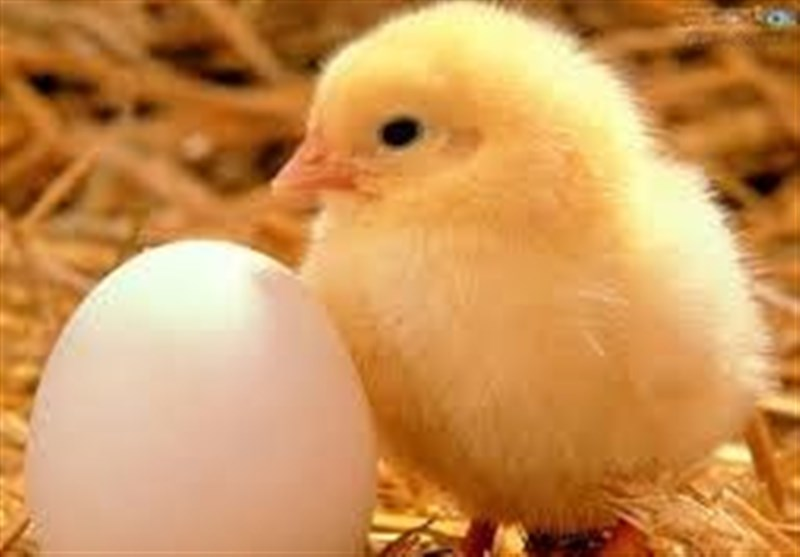
\includegraphics[scale=0.3]{1.jpg}
\end{center}

\newpage
\section{Formula}
\begin{center}
    {\Large
       $$ \sum_{a}^{b}= \int_{2}^{b} \binom{13}{5} $$
    } 
\end{center}

\section{Table}
\begin{table}[h]
    \begin{center}
         matrix: \\
         \setstretch{1}
        \begin{tabular}{||c|c|c|c||}
            \hline
            1 & 2 & 3 & 4\\
            \hline
            2 & 3 & 4 & 1\\
            \hline
            3 & 4 & 1 & 2\\
            \hline
             4 & 1 & 2 & 3\\
            \hline
        \end{tabular}
    \end{center}
\end{table}

\newpage
\section{Code}
ugly c++ :)\\
\begin{lstlisting}[language=C++]
    #include <bits/stdc++.h>
    
    using namespace std;
    
    inline void getAnswer(){
        cout << "It My Oslab HomeWork" << endl ;
    }
    
    inline void getName(){
        cout << "Mahsa KhoMohammadi" << endl ;
    }
    
    int main()
    {    
        getName();
        getAnswer();
        return 0;
    }
\end{lstlisting}

\end{document}
